\section{Modelo usando el dataset VarQ}

Comenzamos nuestro trabajo analizando el dataset construido en la tesis de Santiago Moreno. Este dataset fue construido inicialmente con las variantes originales del sitio de VarQ, que consistieron en aproximadamente 400 mutaciones correspondientes a 13 proteínas con 10 variables. Posteriormente en el mismo trabajo se aumentó la cantidad para llegar a las aproximadamente 18 mil variables del dataset VarQ usando otras fuentes como Clinvar y Humsavar. Llamaremos a este dataset \textit{VarQ Completo}. 

\subsection{Variables del dataset VarQ Completo}

A continuación damos una descripción detallada de las variables originales encontradas en el dataset \todo{CITAR SANTI Y MODIFICAR}. 

\begin{itemize}
    \item Variación de Energía (ENE): En \textit{VarQ}, las mutaciones son modeladas con el software FoldX, construye un modelo a partir de una estructura dada, mutando residuos específicos. El software predice el impacto energético de la mutación en la estabilidad de la proteína o, en caso de tratarse de un complejo, en la estabilidad del mismo.
    \item SASA : Es el valor correspondiente a la superficie accesible por parte del solvente, de la cadena lateral del aminoácido. Este valor permite determinar si la cadena lateral se encuentra en la superficie o en el núcleo de la estructura.
    \item Porcentaje de SASA: El porcentaje que representa el SASA sobre el total. Es decir el porcentaje que representa el SASA en función de la estructura de la proteína.
    \item B-Factor (BF): o factor de temperatura, que corresponde a un aminoácido dentro de la proteína. Una mayor temperatura, indica que el aminoácido pertenece a una zona potencialmente de mayor movilidad.
    \item Switchability (SWI): Evalúa cuán propenso a generar un cambio de hélice alfa a hoja beta es un conjunto de aminoácidos.
    \item Aggregability (AGG): El software Tango evalúa cuán
    propenso es un aminoácido a generar agregación en una proteína desde un punto de vista estructural. La agregación es el proceso por el cual proteínas mal formadas
    adoptan una conformación que causa su polimerización en fibrillas agregadas y organizadas. Muchas enfermedades neurodegenerativas (Amiloidosis) están asociadas con la agregación proteica.
    \item Conservación (CONS): Se calcula en bits, siempre y cuando la mutación pueda ser mapeada a una posición en una familia PFam asignada. Cuando una posición tiene un alto valor en bits y la
    misma posición coincide con el aminoácido conservado en la secuencia de la proteína
    interpretamos que dicha posición está altamente conservada. La misma puede estar
    altamente conservada porque es importante estructuralmente o porque es importante para
    la actividad enzimática. Los residuos con alta conservación tendrán un impacto mayor sobre la función pues afectan aminoácidos de la familia.
    \item Sitio Activo (AS): Las posiciones de sitio activo son
    aquellas que se encuentran marcados como unidos a ligandos en los archivos PDB o que
    pertenecen al mismo pocket que se encuentren conteniendo estos residuos nombrados o
    aquellos que pertenezcan al Catalytic Site Atlas.
    \item Interfaz 3DID: Determina si la posición sirve para una interfaz proteína-proteína según la base de datos de 3DID.
    \item Interfaz PDB: Determina si la posición sirve para una interfaz proteína-proteína según la base de datos de PDB.
\end{itemize}


\subsection{Limpieza del dataset VarQ Completo}

Para trabajar con este dataset decidimos verificar la etiqueta de cada una de las variantes, para confirmar que su status siguiera vigente. Para esto recurrimos a las fuentes Clinvar y Humsavar. Realizamos un primer filtrado de estas tablas quedándonos con aquellas variables con un status confirmado: en el caso de Humsavar, aquellas que figuran con la expresión \textit{Polymorphism} y \textit{Disease}, mientras que en Clinvar nos quedamos con aquellas que figuraban como \textit{Benign} y \textit{Pathogenic}, eliminando aquellas con caracterización difusa, por ejemplo, ``factor de riesgo''. 

\begin{figure}[H]
    \centering
    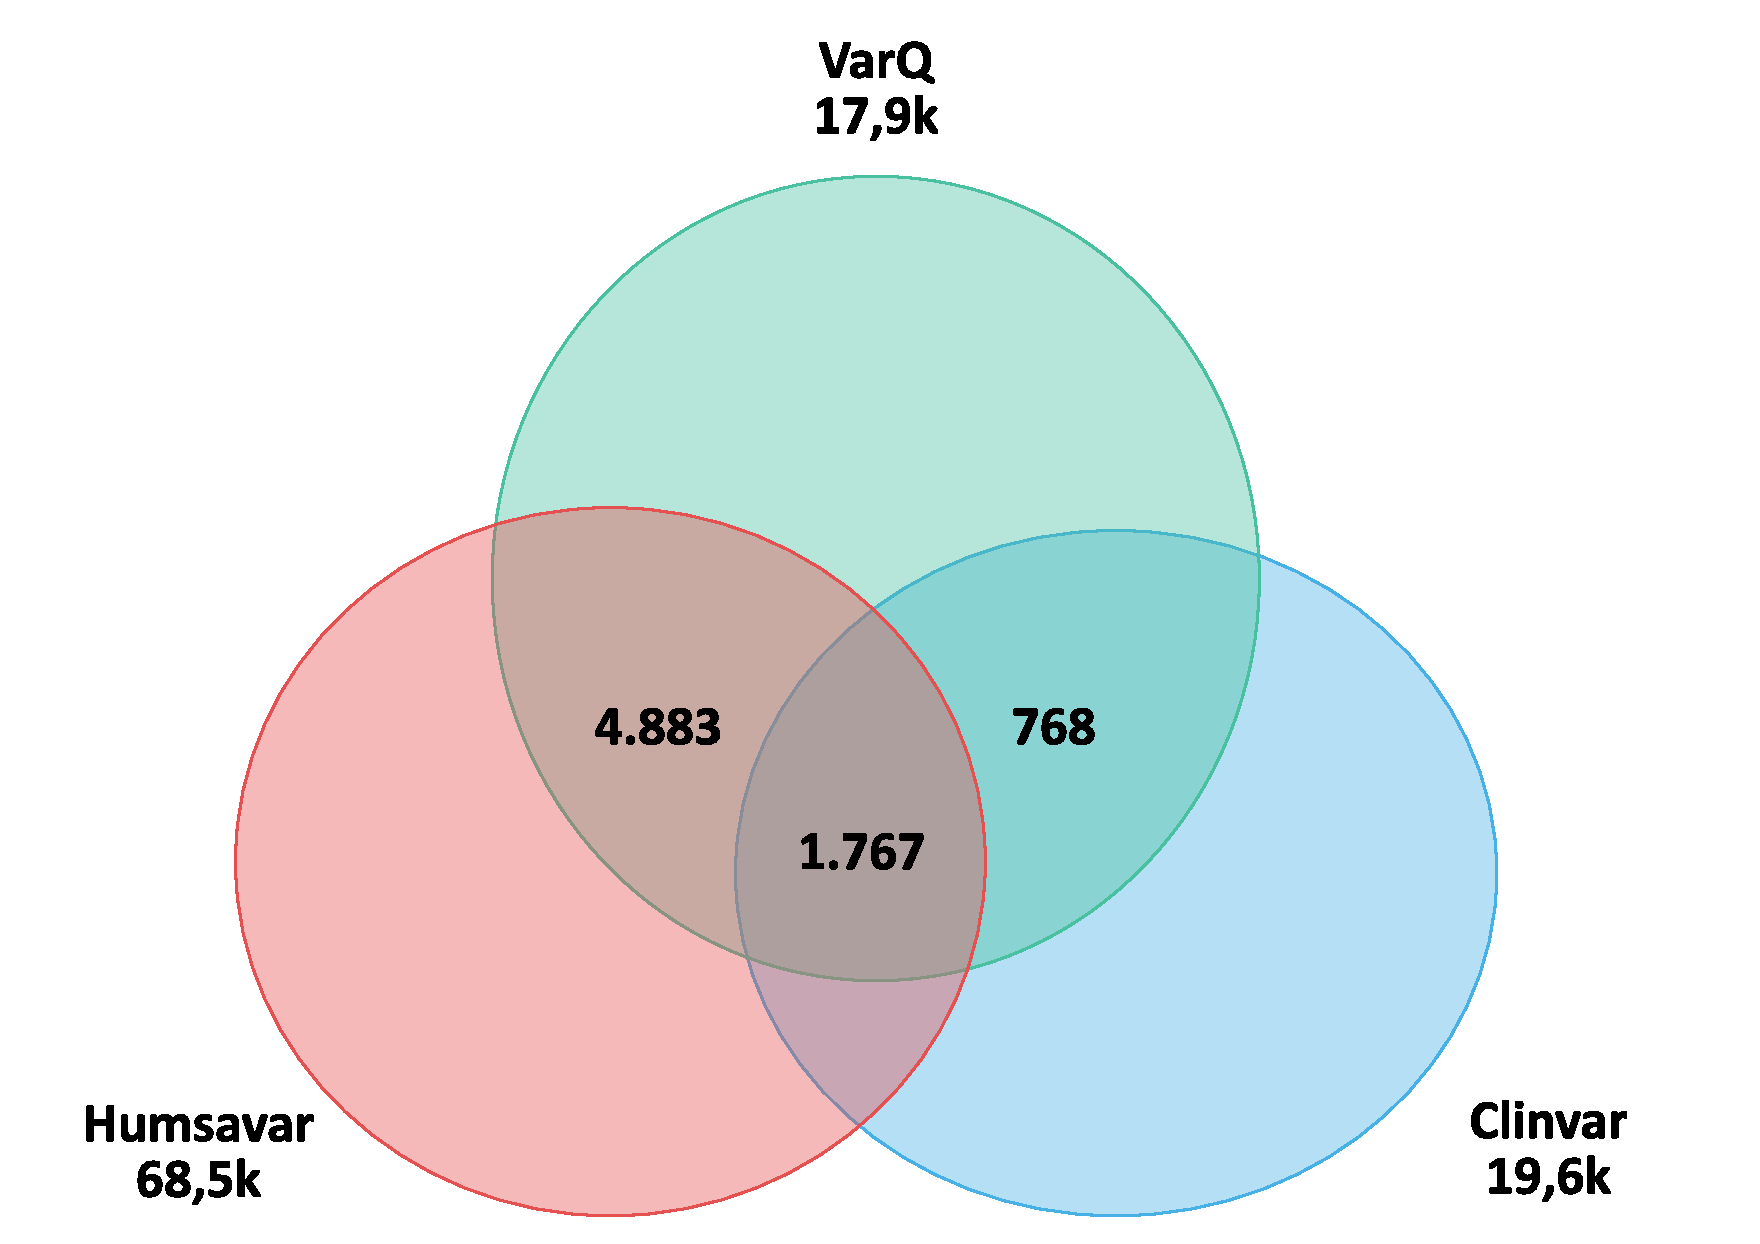
\includegraphics[scale=0.4]{documents/latex/figures/3/interseccion_varq.pdf}
    \caption{Valores en la intersección del dataset VarQ con las tablas Clinvar y Humsavar.}
    \label{fig:interseccion_varq}
\end{figure}

Así, cruzamos los datos con las tablas filtradas Humsavar y Clinvar, y encontramos un subconjunto importante de variantes que no aparecían en ninguna de las dos fuentes. Estas variantes estaban rotuladas en su gran mayoría (94\%) como benignas, por lo que creemos que se consideraron como variantes benignas a todas aquellas a las que no se encontró un reporte. Decidimos remover estas variantes del dataset por considerar que si alguna de ellas está rotulada incorrectamente va a generar ruido. Como puede observarse en la figura 3.1, de las 17.869 variantes del dataset, logramos encontrar 2.535 en la tabla de Clinvar, de los cuales sólo 2.397 tenían un estado confirmado como patogénicas, y 138 como benignas. Cruzando el dataset con la tabla Humsavar encontramos una intersección de 6.650 variantes de los cuales 4.667 corresponden a patogénicas y 1.983 son benignas. Decidimos mantener la clasificación de Humsavar en la intersección de los tres conjuntos por considerarla de mayor confiabilidad dado que es un reporte único curado por expertos a diferencia de Clinvar que es una recopilación de variantes de diversa significación clínica. Esto nos deja con un dataset reducido de 7.418 variantes de las cuales 5.377 son patogénicas y 2.041 son benignas. Denominaremos a este dataset \textit{VarQ Reducido}. 


\subsection{Descripción estadística del dataset VarQ Reducido}

A partir de VarQ Reducido estudiaremos sus variables usando estadísticas descriptivas con el objetivo de evaluar la calidad del dataset. La idea es poder tener una noción de la posición y la dispersión de nuestros datos, sumado a la cobertura que tenemos de ellos sobre las variantes. En la tabla 1.1 podemos ver distintas métricas sobre las variables continuas del dataset como la cantidad de variables con valor no nulo (count), la media de los valores (mean), el desvío estándar (std), el valor máximo (max) y los cuartiles. 

\begin{table}[H]
\centering
\begin{tabular}{|l|l|l|l|l|l|l|l|}
\hline
 & SASA & SASA\% & BFACTOR & SWITCH & AGG & CONS & ENE \\ \hline
count & 7070.0 & 7070.0 & 7070.0 & 6704.0 & 5335.0 & 2742.0 & 7418.0 \\ \hline
mean & 32.11 & 0.15 & 56.45 & 0.38 & 5.02 & 0.33 & 2.91 \\ \hline
std & 39.15 & 0.18 & 71.76 & 0.89 & 17.61 & 0.19 & 4.84 \\ \hline
min & 0.0 & 0.0 & 0.0 & 0.0 & 0.0 & 0.13 & -12.64 \\ \hline
25\% & 0.67 & 0.0 & 19.77 & 0.0 & 0.0 & 0.25 & 0.26 \\ \hline
50\% & 15.21 & 0.07 & 37.34 & 0.01 & 0.0 & 0.3 & 1.51 \\ \hline
75\% & 52.15 & 0.27 & 61.14 & 0.28 & 0.16 & 0.37 & 3.89 \\ \hline
max & 246.41 & 0.75 & 755.61 & 8.72 & 100.0 & 4.77 & 57.51 \\ \hline
\end{tabular}
\caption{Descripción de variables del dataset VarQ Reducido.}
\end{table}

Por otro lado también estamos interesados en detectar variables con muy poca cobertura. En la figura 1.2 podemos observar como la variable de sitio activo (ACTIVE\_SITE) no posee datos para casi ninguna variantes (aproximadamente el 95\%), mientras que la variable de conservación (CONS) no posee datos para el 63\% de las variantes. En base a estas observaciones decidimos remover la variable de sitio activo del dataset por considerarla muy poco relevante en términos de cobertura.

\begin{figure}[H]
    \centering
    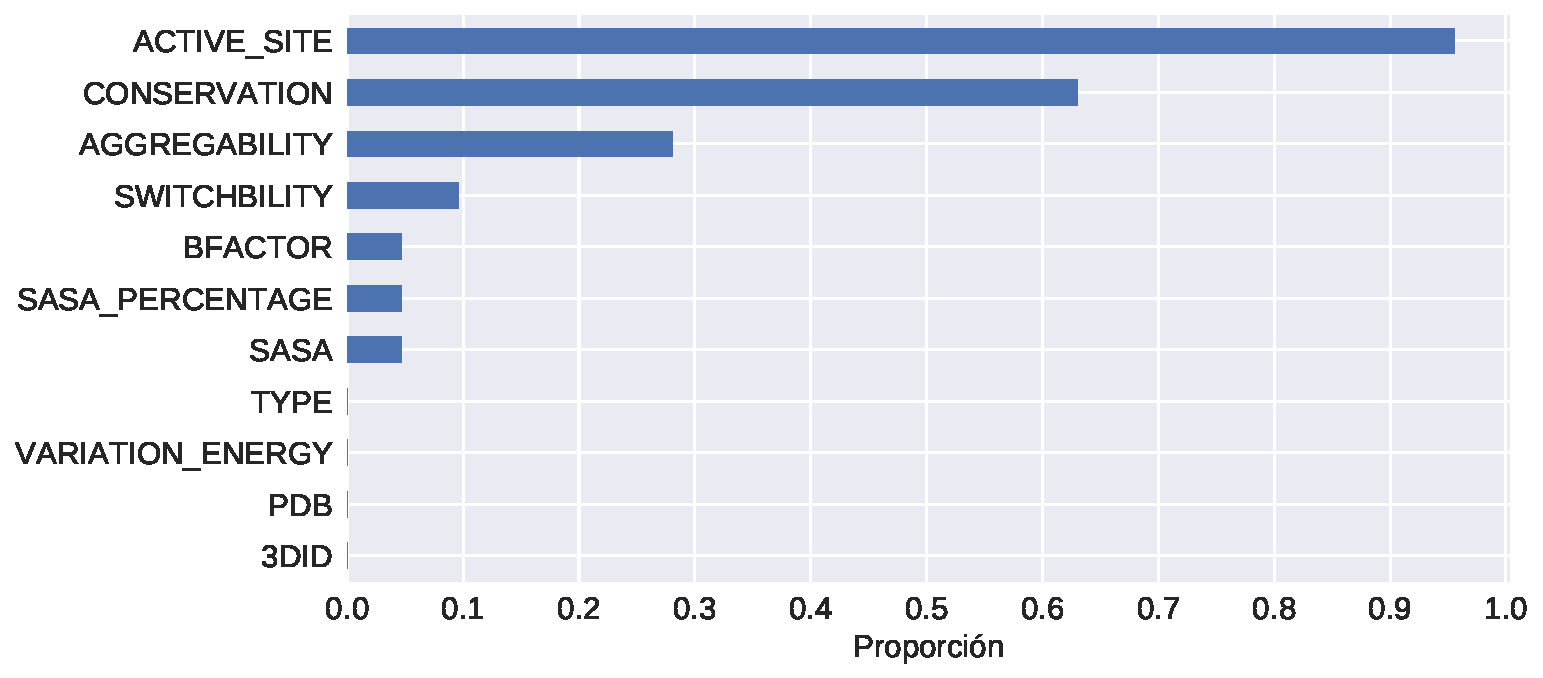
\includegraphics[scale=0.55]{documents/latex/figures/3/proporcion_nulos.pdf}
    \caption{Proporción de variantes con valor nulo por variable del dataset VarQ Reducido.}
    \label{fig:proporcion_nulos_varq}
\end{figure}

Por último, queremos saber cuantas variables nulas tienen cada una de las variantes del dataset. En la figura 1.3 podemos observar que existe aproximadamente un 5 \% de variantes que poseen 7 variables nulas de las 10 que contienen el dataset, es decir, prácticamente no tienen ningún tipo de información, y sólo el 2\% de las variantes posee el total de las variables cubiertas. Por el otro lado, casi el 90\% de las variantes tiene a lo sumo 3 variables nulas.

\begin{figure}[h]
    \centering
    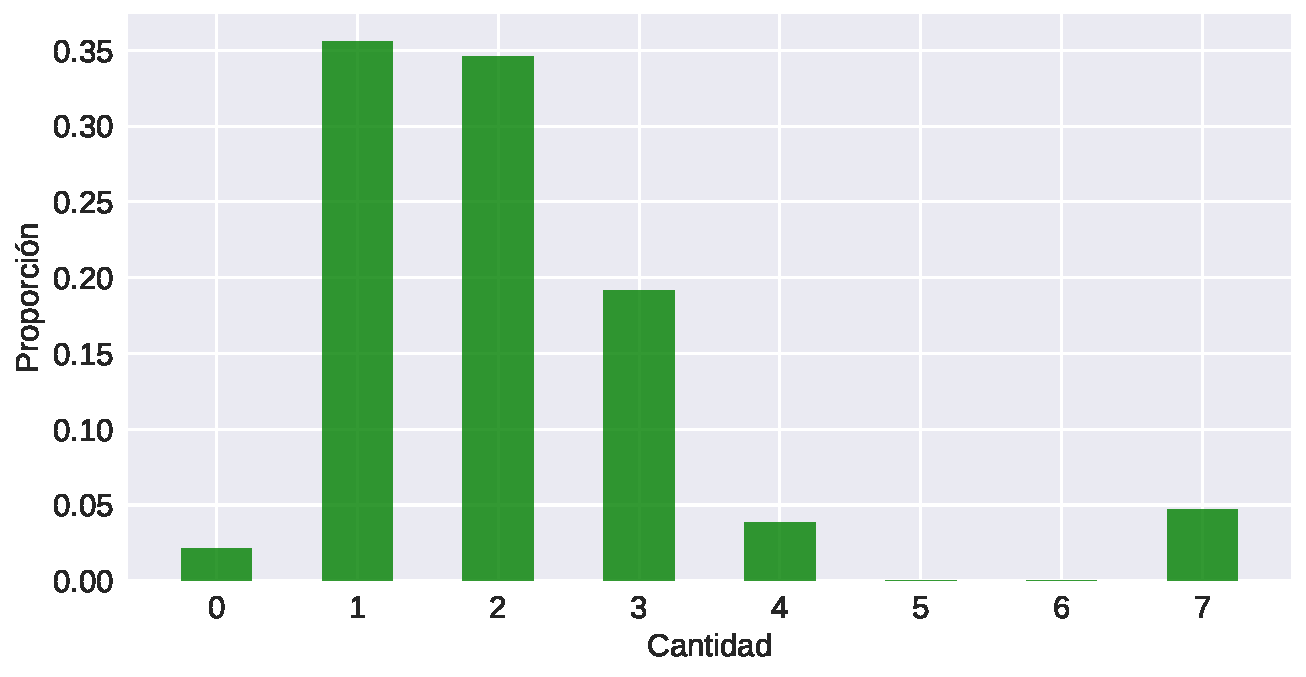
\includegraphics[scale=0.55]{documents/latex/figures/3/nulos_varq.pdf}
    \caption{Histograma de cantidad de variables nulas del dataset VarQ Reducido.}
    \label{fig:nulos_varq}
\end{figure}


\subsection{Modelo creado a partir del dataset Reducido}

Una vez definido el dataset, podemos generar un modelo estadístico.


Si bien la cantidad de variantes patogénicas es mucho mayor que la cantidad de variantes benignas (es decir, el dataset se encuentra desbalanceado) decidimos generar un modelo para poder evaluar de forma superficial la dificultad del problema. Decidimos probar diferentes modelos (SVM, Regresión Logística y Random Forest) (\todo{Mostrar gráfico del rendimiento de cada modelo}), imputando la variables nulas con la mediana y estandarizando, y obtuvimos los mejores resultados en el caso del Random Forest. Cómo se puede observar en la figura 3.2 se obtuvo un AUC de 0,68. 

% Dado que la cantidad de variantes patogénicas en el dataset VarQ reducido es mucho mayor que la cantidad de variantes benignas decidimos generar 10 datasets distintos con las 2 mil variantes benignas y un subset aleatorio de 2 mil variantes patogénicas para obtener un conjunto de datasets balanceado de entrenamiento. Los resultados del algoritmo aplicado en cada uno de los datasets se promedió y se tuvo en cuenta la variación entre los resultados al momento de ser reportados. 
% En cada uno de los datasets se dividieron las variantes en subsets de entrenamiento (2/3 del total) y test (1/3 del total). Se entrenó con distintos algoritmos (Random Forest, Regresión Logística y Support Vector Machine), obteniendo el mejor resultado en el Random Forest. La curva AUC 


\begin{table}[H]
\centering
\begin{tabular}{|l|l|l|l|}
\hline
              & Precisión & Recall & F1-score \\ \hline
Patogénicas   & 0.62      & 0.27   & 0.38     \\ \hline
Benignas      & 0.71      & 0.92   & 0.80     \\ \hline
Promedio      & 0.68      & 0.69   & 0.65     \\ \hline   
\end{tabular}
\caption{Reporte de métricas del modelo usando el dataset VarQ.}

\label{fig:metrics_varq}
\end{table}

\begin{figure}[h]
    \centering
    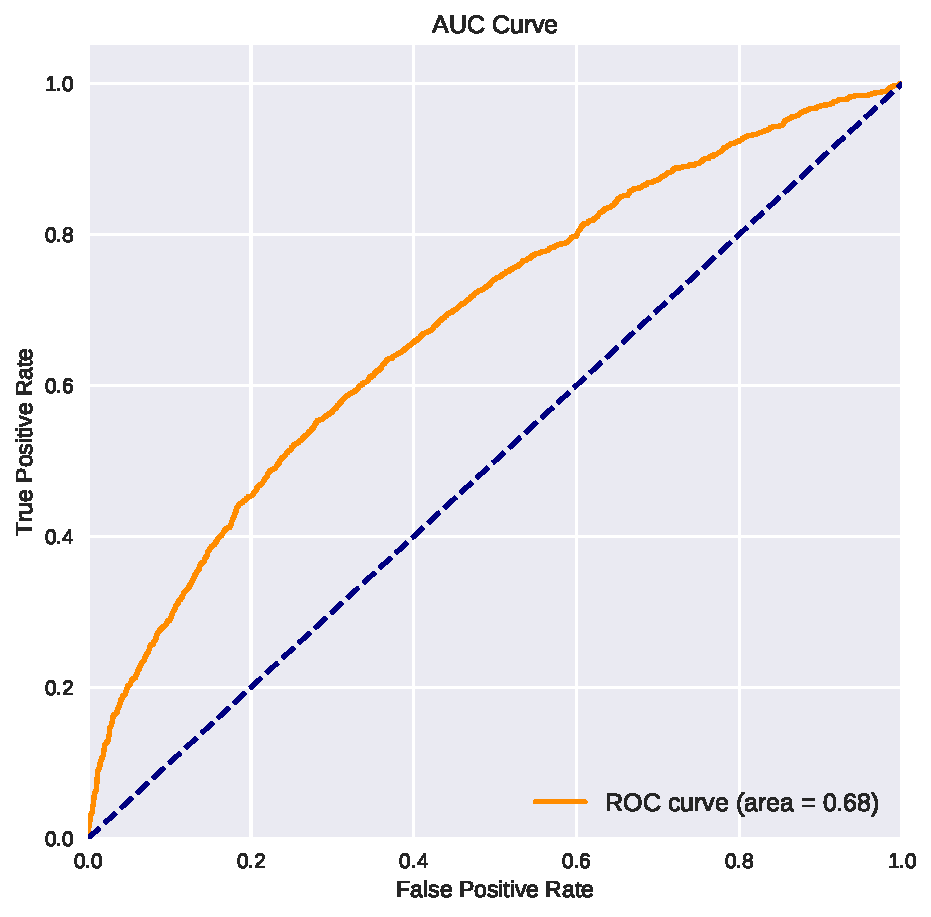
\includegraphics[scale=0.55]{documents/latex/figures/3/auc_varq.pdf}
    \caption{Curva AUC del algoritmo Random Forest del dataset VarQ. La línea punteada corresponde a un predictor Random. \todo{Correr para el nuevo dataset}}
    \label{fig:auc_varq}
\end{figure}

En la figura 3.3, la importancia de los features reportado por el algoritmo Random Forest puso en primer lugar con una gran diferencia a la variable que hace referencia al impacto energético de la mutación.  

\begin{figure}[H]
    \centering
    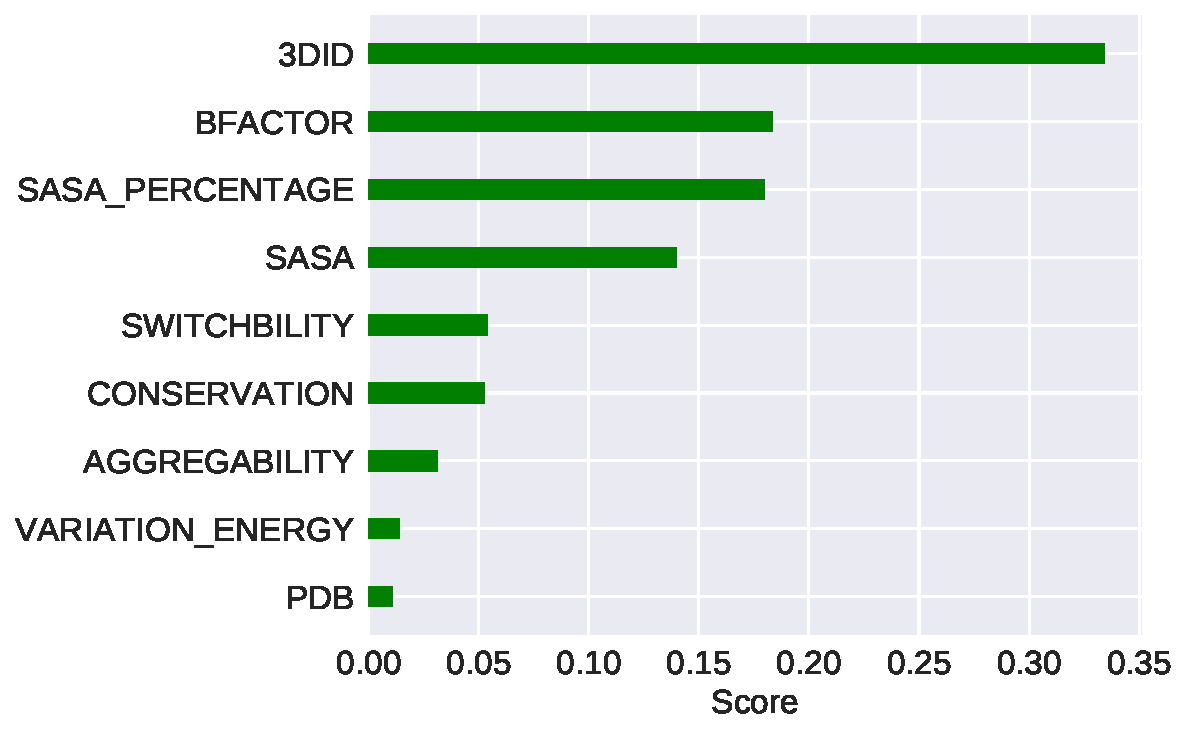
\includegraphics[scale=0.55]{documents/latex/figures/3/importances_varq.pdf}
    \caption{Los atributos más importantes del dataset VarQ usando un modelo Random Forest. \todo{Correr para el nuevo dataset}}
    \label{fig:importance_varq}
\end{figure}

\section{Modelo usando Propiedades Estructurales de la Proteína}

En esta sección generamos un nuevo dataset utilizando las variantes de Humsavar (a nivel de proteínas) buscando nuevas fuentes de información de carácter estructural de las proteínas.

Para el análisis de estas variable usamos el dataset de variables de Humsavar, que se compone de 68523 variantes (o ``mutantes'') de las cuales 39655 son variantes benignas (58\%) y 28868 (42\%) están asociadas a enfermedades. 

\subsection{Extracción de variables usando Biopython}

La primer fuente que utilizamos por su relativa facilidad en la extracción de un conjunto de variables físico químicas de la proteína fue el módulo ProtParam de la biblioteca Biopython. Esta biblioteca es un set de herramientas escritas en Python desarrollada por colaboradores para el área de la bioinformática, y posee una licencia de uso libre \todo{[citar]}.
El nombre ProtParam proviene de \textit{Protein Parameters} (parámetros de la proteína) y está basado en la herramienta del server proteómico Expasy \todo{[citar]}. Requiere el \textit{accession number} de la proteína (identificador único) o una subsecuencia de la misma para poder acceder a los parámetros calculados \todo{[citar]}, que son los siguientes:

\begin{itemize}
    \item Peso molecular
    \item pI Teórico
    \item Composición aminoácida
    \item Composición atómica
    \item Coeficiente de extinción
    \item Período de semi-desintegración o hemivida
    \item Índice de instabilidad
    \item Índice alipático
    \item Promedio de hidropaticidad
\end{itemize}

Para poder utilizar el módulo entonces recurrimos a Uniprot para conseguir el proteoma humano en formato FASTA. El formato FASTA fue desarrollado por David Lipman y William Pearson en 1985, y originalmente fue incluido en un programa del mismo nombre utilizado para el alineamiento múltiple de secuencias. Una archivo FASTA puede incluir diferentes secuencias, no necesariamente de aminoácidos, y cada una de estas secuencias posee una línea de descripción al comienzo que empieza con el símbolo $>$ \todo{[citar]}. Por ejemplo:

\begin{verbatim}
	>P01013 GENE X PROTEIN (OVALBUMIN-RELATED)
	QIKDLLVSSSTDLDTTLVLVNAIYFKGMWKTAFNAEDTREMPFHVTKQESKPVQMMCMNNSFNVATLPAE
	KMKILELPFASGDLSMLVLLPDEVSDLERIEKTINFEKLTEWTNPNTMEKRRVKVYLPQMKIEEKYNLTS
	VLMALGMTDLFIPSANLTGISSAESLKISQAVHGAFMELSEDGIEMAGSTGVIEDIKHSPESEQFRADHP
	FLFLIKHNPTNTIVYFGRYWSP
\end{verbatim}


A partir del proteoma obtenido se extrajeron las secuencias correspondientes a las proteínas del dataset Humsavar, y para cada una de ellas se tomó una subsecuencia de la misma alrededor de la posición donde se produjo la variante.

\vspace{2mm}
\todo{
TODO: Esquema de la subsecuencia
}
\vspace{2mm}

Para cada una de los parámetros calculados en ProtParam, generamos dos variables que buscan reflejar la diferencia generada por la variante. \todo{TODO: Hablar de los métodos usados}.

\subsection{Extracción de variables usando SNVBox}

Además de la información obtenida vía ProtParam, recurrimos a una base de datos llamada SNVBox. Esta base de datos fue elaborada y es actualmente mantenida por el Karchin Lab de Universidad Johns Hopkins. Se encuentra en su versión 3.0 y sigue en desarrollo. \todo{Mencionar algunos papers que usaron esta base}. SNVBox posee alrededor de 90 variables consideradas relevantes para detectar el impacto biológico de un SNV \cite{Wong2011}, como datos sobre la estructura de la proteína, a nivel de aminoácido y también a nivel de los sitios de la proteína donde se encuentra la variante. Otra característica destacable de esta fuente es que posee dichas variables para todos los codones del exoma humano, lo que nos permitió una cobertura alta para las variantes del dataset con el que trabajamos.
Algunas de las variables encontradas fueron:

\vspace{2mm}
\todo{
TODO:
1. Lista de variables
2. Diagrama de SNVBOX
}
\vspace{2mm}

\subsection{Descripción del \textit{Dataset Estructural}}

Luego del proceso del extracción de variables generamos un nuevo dataset cruzando estos atributos con las variantes de Humsavar. En el caso de los atributos relativos a los aminoácidos, pudimos cruzarlos usando la columna del dataset referente al identificador de la proteína, la posición de la variante, y el par de aminoácidos que se intercambiaron. Con los atributos relativos al genoma, pudimos cruzar la información usando la columna RSID (Reference SNP cluster ID). Esta columna identifica a un cluster de variaciones de un sólo nucleótido que pertenece a la misma posición en el genoma (o conjunto de posiciones) \cite{Ostell2007}. 
El dataset resultante (denominado \textit{Dataset Estructural}) está compuesto por 68,5 mil variantes y 28 variables incluyendo la variable de respuesta (o tipo), de los cuales 39,6 mil son benignas (no se encontraron reportes de enfermedades en la literatura), y 28,8 mil variantes están asociadas a alguna enfermedad. 
Una de las formas que nos permite ver que tan bien las variables de este dataset están separando nuestros tipos de SNPs, es usar reducción de dimensionalidad. El primer método que probamos fue el análisis de componentes principales (PCA), con el que generamos dos componentes, que son combinaciones lineales de nuestras variables iniciales de forma de maximizar la varianza, es decir el par de componentes que mejor explican la información completa.

\todo{TODO: Poner gráfico de PCA}

\subsection{Generación del Modelo}

Con este dataset generamos un modelo basado en un predictor Random Forest. Para la búsqueda de hiperparámetros usamos \textit{Grid-Search} (búsqueda ``en cuadrícula''). \todo{TODO: Evaluar RandomSearch}. Las variables se imputaron usando la mediana, y no fueron escalados al no ser necesario en algoritmos de clasificacion basados en árboles de decisión, dado que se evalúan las variables de forma independiente (\todo{cita?}). Se eligió inicialmente este tipo de predictor por ser el que obtuvo los mejores resultados en el dataset VarQ  con respecto a otros predictores (SVMs y Regresión Logística) y para centrar el análisis en cómo las variables afectan al modelo.  

Como puede observarse en la figura 3.4, a partir de este modelo se obtuvo un AUC de 0,71, que supera lo obtenido por el modelo usando el dataset VarQ. Las métricas observadas en la tabla 3.2 permiten dar cuenta de una precisión del 34\% con respecto a las variantes patogénicas, es decir, el modelo está reportando una 66\% cantidad de variables como patogénicas que no lo son (también conocido como error de tipo I), y un recall de 63\%, lo que indica que existe un 34\% de variables patogénicas en nuestro dataset que no están siendo detectadas por nuestro modelo (error de tipo II). \todo{TODO: Diagrama de errores}.

\begin{table}[H]
\centering
\begin{tabular}{|l|l|l|l|}
\hline
              & Precisión & Recall & F1-score \\ \hline
Patogénicas   & 0.34      & 0.63   & 0.44     \\ \hline
Benignas      & 0.88      & 0.67   & 0.76     \\ \hline
Promedio      & 0.76      & 0.67   & 0.70     \\ \hline
\end{tabular}
\caption{Métricas del modelo Random Forest aplicado al dataset estructural.}
\label{my-label}
\end{table}

% \subsection{Resultados}

\begin{figure}[h]
    \centering
    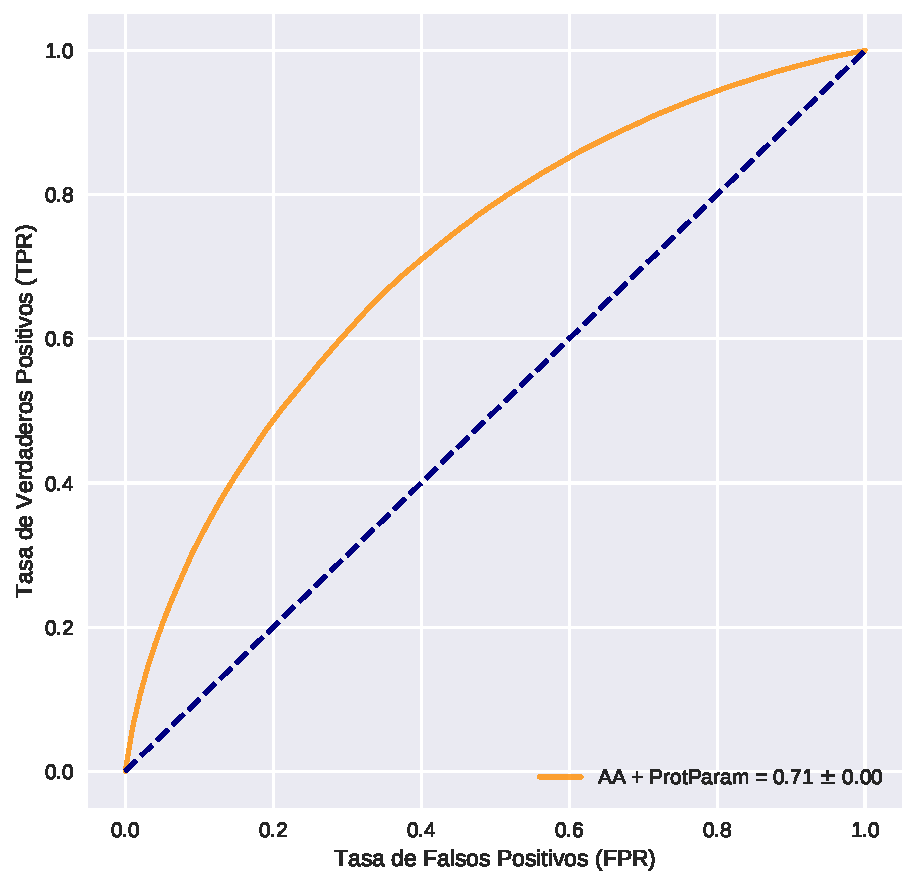
\includegraphics[scale=0.55]{documents/latex/figures/3/auc_1.pdf}
    \caption{Curva AUC del algoritmo Random Forest aplicado al dataset estructural. La línea punteada corresponde a un predictor Random.\todo{TODO: Correr modelo con un solo set train y test.}}
    \label{fig:auc_1}
\end{figure}

% \subsection{Importancia de los atributos}

El algoritmo nos permite identificar los mejores atributos dado su rango en cada uno de los árboles del clasificador. En este caso, podemos ver que los primeros tres atributos refieren a matrices de sustitución. Los siguientes features pertenecen a ProtParam, como la aromaticidad, la flexibilidad y la hidrofobicidad. La hidrofobicidad, o la capacidad de repeler el agua de la subsecuencia de los aminoácidos, es uno de las variables consideradas relevantes para definir la patogenicidad de una proteína, de acuerdo a \cite{Wang2016}. Por el otro lado, podemos observar variables con un nivel de importancia muy similar, como es el caso de PAM25, EX y BLOSUM. Estas variables corresponden a matrices de sustitución, y en la figura 3.6 podemos observar que existe una alta correlación entre ellas. \todo{TODO: Evaluar formas de variar el modelo usando variables que no esten correlacionadas. MRMR?} 

\begin{figure}[H]
    \centering
    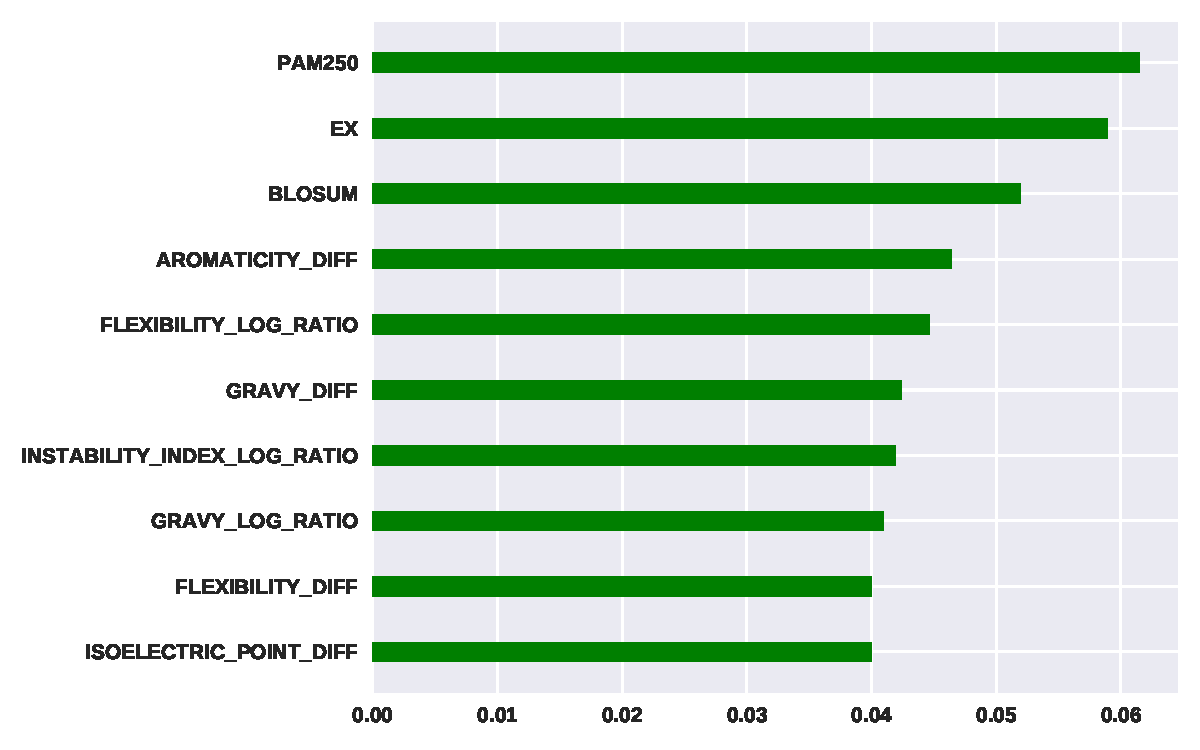
\includegraphics[scale=0.55]{documents/latex/figures/3/importance_1.pdf}
    \caption{Los 10 atributos más importantes del modelo Random Forest usando el dataset estructural. \todo{Falta eje x}}
    \label{fig:importance_1}
\end{figure}

% \subsection{Correlación}

\begin{figure}[H]
    \centering
    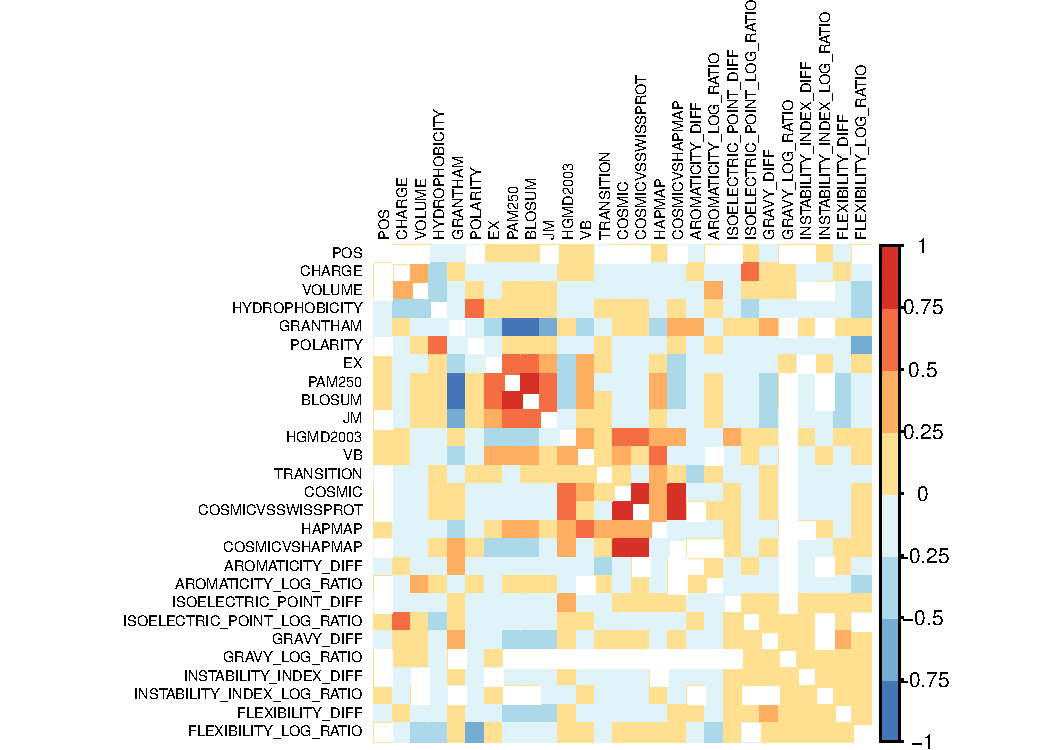
\includegraphics[scale=0.8]{documents/latex/figures/3/corrplot_1.pdf}
    \caption{Test de Correlación de Pearson (Significación: 0,05) sobre las variables del dataset estructural. Los valores en blanco poseen un p-valor por debajo del nivel de significación. Se puede observar que GRANTHAM se encuentra altamente anti-correlacionado con las matrices PAM y BLOSUM, mientras que estas se encuentran correlacionadas al igual que con EX.}
    \label{fig:corrplot_1}
\end{figure}

\section{Modelo usando Variables Genómicas}

Otra de las preguntas que nos hicimos al momento de comenzar este trabajo fue si las variables genómicas podían hacer un aporte al modelo, siendo que en los genes es donde se produce la mutación que finalmente da origen a la variante en la proteína. Como mencionamos preciamente, en la tabla Humsavar existe, para la mayoría de las mutaciones, el RSID o Reference SNP ID. Este identificador agrupa los distintos reportes que hagan referencia a la misma posición dentro del mismo genoma de referencia (hg19/GRCh37). A partir del RSID fue posible la consulta a la base de datos dbSNP (Versión snp150) con el que obtuvimos mayores detalles como ser el cromosoma, la posición y el cambio de nucleótido de la variante. 

En la literatura encontramos que dos de las variables genómicas asociadas a la conservación eran las que daban mejores resultados (modelos FATHMM-MKL \cite{Shihab2015} o VEST \cite{Carter2013}). Esta \textit{conservación} es un término biológico que refiere a las secuencias conservadas, es decir secuencias tanto genéticas como proteicas que se mantienen de forma similar o idéntica a en muchas especies que poseen un ancestro evolutivo en común (esta \textit{familia} de especies también se denomina árbol filogenético). En particular, la composición de estas variables consiste en alineamientos múltiples de secuencias genéticas (MSA) de 46 especies de vertebrados, incluyendo Homo Sapiens y otras como Felis catus (gato doméstico), Danio renus (pez cebra) y Equus Caballus (el caballo). En base a este alineamiento se usan dos medidas distintas de conservación, \textbf{PhastCons} \cite{siepel2005evolutionarily} y \textbf{PhyloP} \cite{Pollard2010}, que buscan detectar aquellas regiones en el genoma con mayor nivel de conservación entre las distintas especies. Decidimos incluir en nuestro dataset ambas medidas de conservación, usando el Table Browser de la Universidad de California, Santa Cruz \cite{Karolchik2004}.

También tomamos en consideración la función de la posición dentro del gen. La base de datos dbSNP define cada SNP de acuerdo a su clase funcional. Si la variación se encuentra cerca del intervalo de un transcripto, pero no en la región codificante, la clase funcional va a depender de la posición de la variación relativa a la estructura del transcripto \cite{Ostell2007}. Por otro lado, si la variación se encuentra en una zona codificante, la clase funcional se va a definir en base a si el alelo de la variación va a resultar en una sustitución sinónima (es decir, el nuevo codón va a formar el mismo aminoácido), una sustitución no sinónima (es decir, el nuevo codón va a formar un aminoácido distinto) o una sustitución sin sentido (en donde la mutación genera un codón de terminación prematuro).
Por último, usamos variables genómicas del dataset SNVBox, que calculan la conservación a 46 vías a nivel de exones, y la cantidad de SNPs conocidos en el exón donde se produjo la variante. \todo{TODO: Describir lista de variables del dataset}


A partir del dataset generado (llamado dataset genómico) podemos observar también como las variables permiten separar el dataset en dos clusters mucho mejor discriminados gracias a una combinación entre PCA y t-SNE.

\todo{TODO: Poner gráficos de PCA y t-SNE}

Luego de una primera aproximación al problema de encontrar las variables patogénicas generamos un modelo basado en Random Forest (volvimos a utilizar este algoritmo debido a los resultados obtenidos en el dataset VarQ y para facilitar la comparación entre datasets). En este caso volvimos a imputar las variables con su respectiva mediana.Por las razones descriptas en el capítulo anterior tampoco se escalaron las variables. Como se puede observar en la figura 3.7 obtuvimos un AUC de 0,89. 
Analizando la importancia de las variables (figura 3.8) en el modelo podemos observar que las variables de conservación están en los primeros dos puestos, confirmando lo obtenido por los trabajos de investigación antes mencionados. Por otro lado, esto genera un interrogante adicional: ¿Cuál es la razón por la que la variable \textit{Conservación} del dataset VarQ no genera un rendimiento similar?


\begin{figure}[H]
    \centering
    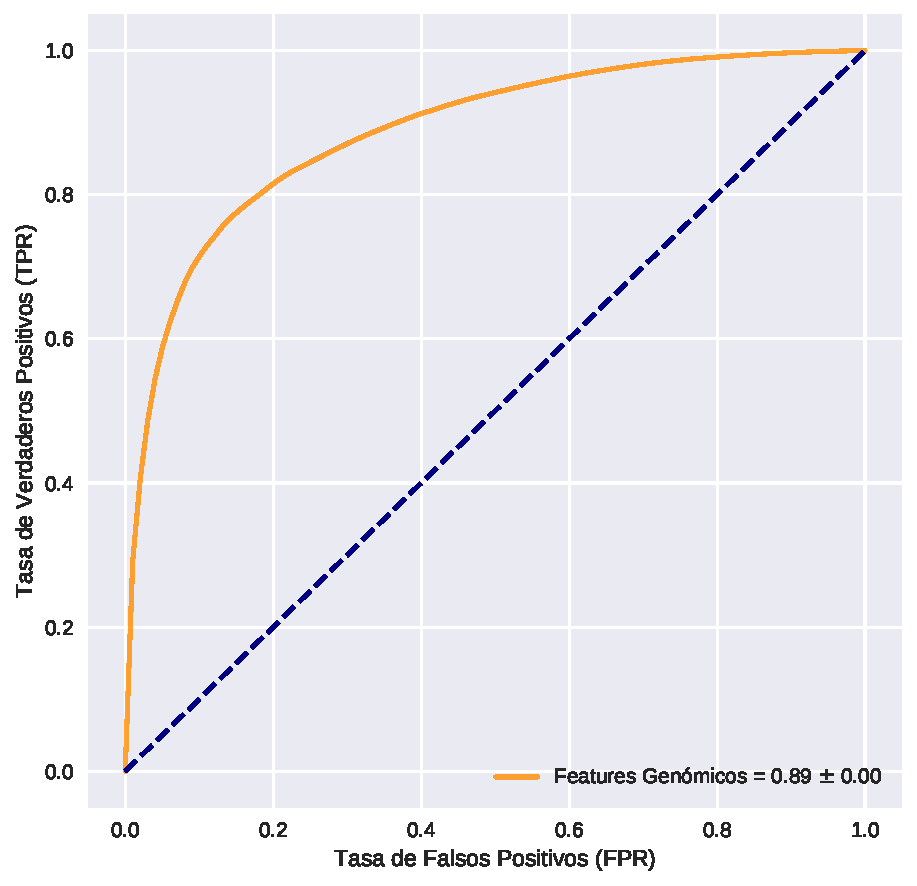
\includegraphics[scale=0.55]{documents/latex/figures/3/auc_2.pdf}
    \caption{Curva AUC del algoritmo Random Forest usando el dataset genómico. La línea punteada corresponde a un predictor Random.}
    \label{fig:auc_2}
\end{figure}

\begin{figure}[H]
    \centering
    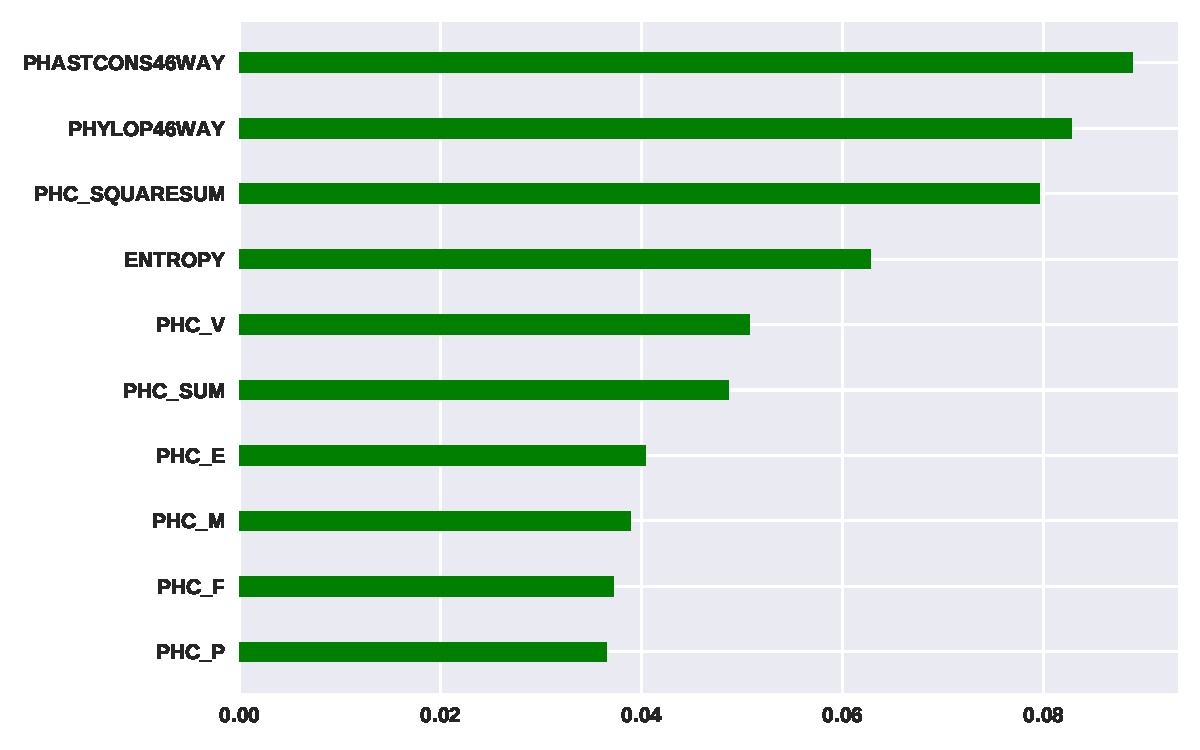
\includegraphics[scale=0.55]{documents/latex/figures/3/importance_2.pdf}
    \caption{Los 10 atributos más importantes del dataset genómico usando un modelo Random Forest. \todo{Falta eje X}}
    \label{fig:importance_2}
\end{figure}

Como podemos observar en la figura 3.8, el poder informativo de las variables de conservación es muy similar. La pregunta que nos hacemos en este caso es: ¿Las dos primeras variables de conservación están en los primeros dos lugares porque están altamente correlacionadas o aportan diferente información sobre las variables? La figura \todo{[x]} da una respuesta afirmativa a esta pregunta \todo{TODO: Hacer gráfico de correlación}. 

\todo{TODO: Gráfico de correlación y observaciones}

% \subsection{Descripción}
% \subsection{Correlación}
% \subsection{Resultados}

\section{Integrando el dataset estructural y el genómico}

Finalmente, unimos los dos conjuntos de variables para ver si representan una mejora frente a los ya excelentes resultados del modelo genómico. El modelo utilizado fue nuevamente Random Forest con imputación usando la mediana. Como se puede observar en la figura 3.9, no hubo una mejora significativa con respecto a los otros modelos. Las variables de conservación siguen encabezando la lista de las variables más importantes del modelo. Una posible hipótesis que explicaría estos resultados es que las variables del dataset genómico terminan ``eclipsando'' las del dataset estructural, y por lo tanto se pierde el subconjunto de variantes detectados por este último. Una forma de observar este efecto es cuantificar dichas variantes, es decir, ver si efectivamente el dataset estructural esta detectando una cantidad significativa de variantes no encontradas por el model genómico que no aparecen en este nuevo modelo. 

\begin{figure}[H]
    \centering
    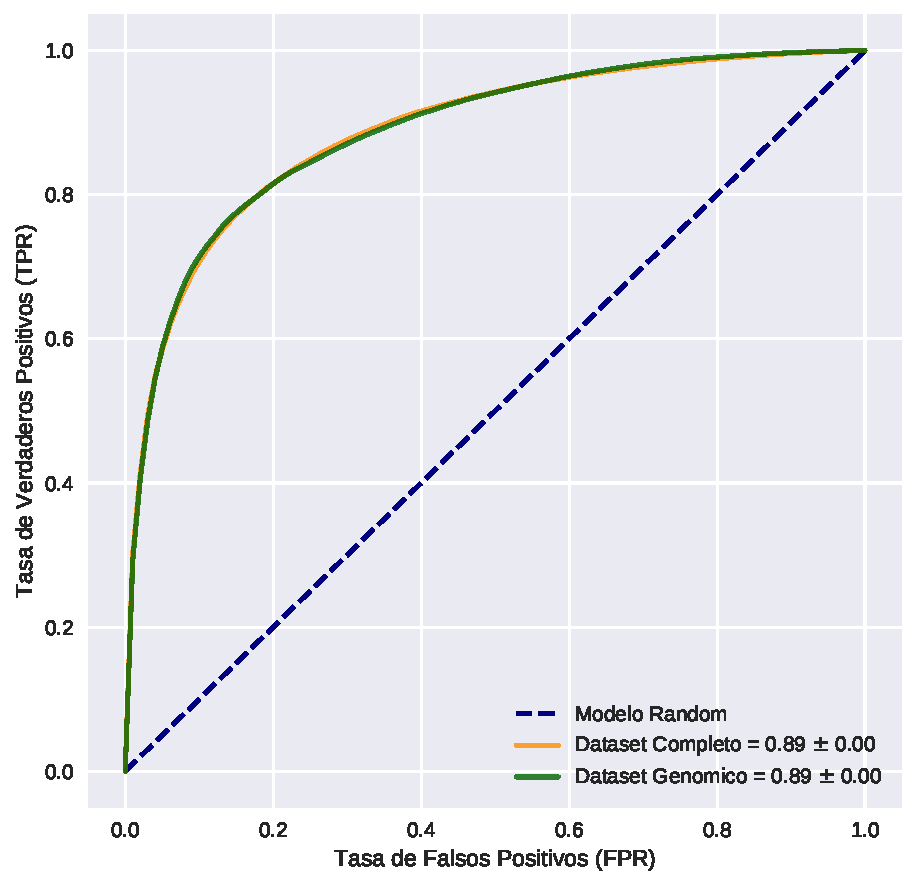
\includegraphics[scale=0.55]{documents/latex/figures/3/auc_3.pdf}
    \caption{Curva AUC del algoritmo Random Forest del dataset integral. La línea punteada corresponde a un predictor Random.}
    \label{fig:auc_3}
\end{figure}

\begin{figure}[H]
    \centering
    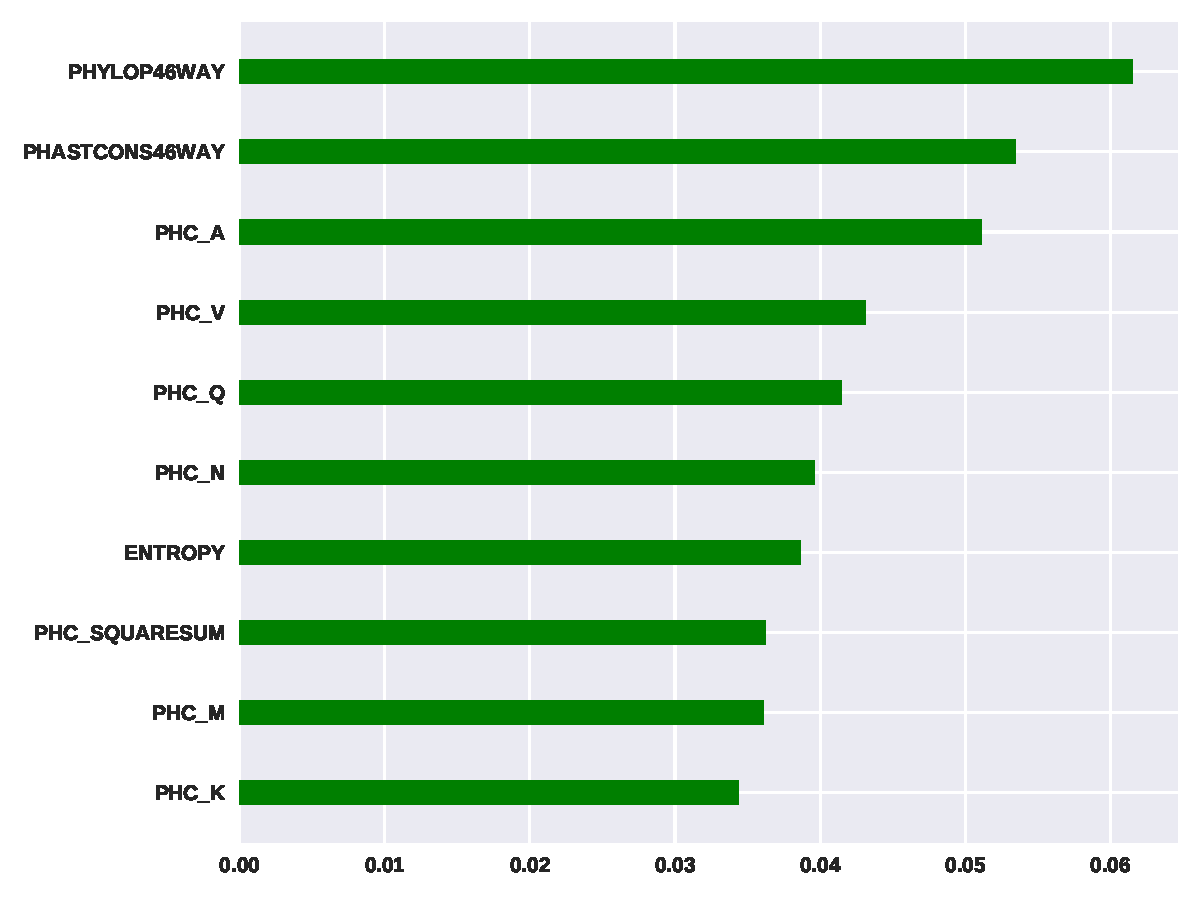
\includegraphics[scale=0.55]{documents/latex/figures/3/importance_3.pdf}
    \caption{Los 10 atributos más importantes del dataset integral.}
    \label{fig:importance_3}
\end{figure}
Una posible hipótesis que explicaría estos resultados es que las variables del dataset genómico terminan ``eclipsando'' las del dataset estructural, y por lo tanto se pierde el subconjunto de variantes detectados por este último. Una forma de observar este efecto es cuantificar dichas variantes, es decir, ver si efectivamente el dataset estructural esta detectando una cantidad significativa de variantes no encontradas por el model genómico que no aparecen en este nuevo modelo.  Ante esta situación una posible solución es usar algún método de ensamble que consiga potenciar al mejor de los dos modelos agregando las demás. Decidimos probar una serie de métodos clásicos de ensambling: Stacking, Bagging, y Boosting.

\todo{TO DO: Explicar métodos y exponer resultados.}
\todo{TO DO: Listar diferencias entre las variantes correctamente detectadas de los dos modelos.}
\todo{TO DO: Cambiar gráficos de AUC, cambiar train-test a uno solo. }

\todo{TO DO: Modificar diccionario de hiperparámetros del RF. Probar brevemente otros métodos para descartar que alguno sea muy superior.}

% \section{Uniendo las variables al Dataset VarQ}

% La siguiente pregunta es si el modelo mejora aún más sumando las variables de VarQ al conjunto de variables con los que trabajamos.


